\documentclass[../main.tex]{subfiles}
\begin{document}

The plan is to show all finitely generated reflection groups are in fact Coxeter groups, which admit a nice geometric classification. This follows\cite{Humphreys1990}

\subsection{Coxeter groups}

\begin{definition}
    We call a group $W$ \textbf{Coxeter} if it admits a presentation of the form:\[
    \abr{r_1,\ldots,r_n \mid (r_ir_j)^{m_{ij}}\text{ for all }i,j}
    \]
    where each $m_{ij}\in \bN\cup\{\infty\}$, and $m_{ii}=2$ for all $i$. For formal reasons, we will consider the pair $(W,R)$, where $R$ is the set of generators in the presentation, and call this a \textbf{Coxeter system}. We call a Coxeter system finite if $R$ is finite.
\end{definition}

To any finite Coxeter system $(W,R)$ we can associate an undirected graph called its \textbf{Coxeter diagram} by the following rules:\begin{itemize}
    \item Draw a node $i$ for each $r_i\in R$;
    \item For each relation $(r_i r_j)^{m_{ij}}$ with $m_{ij}>2$ draw an edge between $i$ and $j$ and label it with $m_{ij}$.
\end{itemize}

This process can be reversed to obtain a Coxeter system from any Coxeter diagram. This correspondence will associate the graph:
\begin{figure}[!h]
\centering
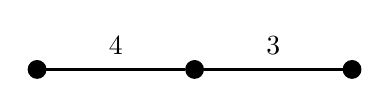
\begin{tikzpicture}
    \begin{scope}[every node/.style={circle, fill=black, draw, thick, minimum size = 6pt, inner sep=0pt}]
        \node (1) at (0,0) {};
        \node (2) at (2,0) {};
        \node (3) at (4,0) {};
    \end{scope}

    \begin{scope}[every edge/.style={draw,very thick}]
        \path [-] (1) edge (2);
        \path [-] (2) edge (3);
        \node at (1,0.3) {$4$};
        \node at (3,0.3) {$3$};
    \end{scope}
\end{tikzpicture}
\end{figure}

to the group presentation: \[
\abr{r_1,r_2,r_3 \ \middle| \ r_1^2 = r_2^2 = r_3^2 = e, \ (r_1r_2)^4 = (r_2r_3)^3 = (r_1r_3)^2 = e}
\]

which happens to correspond to the symmetry group of the octahedron.


\subsection{The fundamental domain}

\subsection{Words}

\subsection{Classification}

\end{document}